\chapter{Проектирование архитектуры и выбор средств решения} \label{ch4}
Для реализации интерактивного визуализатора моделей программ необходимо решить следующие подзадачи:
\begin{itemize}
\item Получение из исходного кода метода на языке Java абстрактного синтаксического дерева
\item Обеспечение отрисовки деревьев и графов в браузере
\item Преобразование структуры AST в данные для отрисовки AST, CFG, DDG, PDG, ASG и SSA
\item Создание интерфейса для взаимодействия с программой
\end{itemize}
\begin{figure}[h]
	\center
	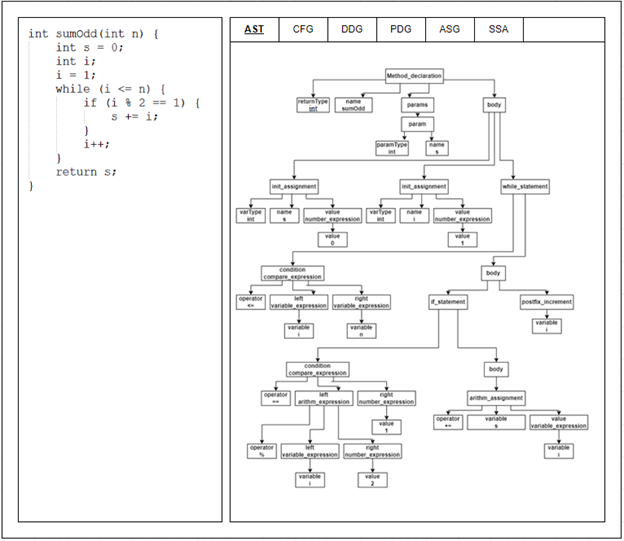
\includegraphics [scale=0.75] {my_folder/images/my/12}
	\caption{Схематичное представление интерфейса визуализатора} 
	\label{fig:12}  
\end{figure}
\section{Парсинг кода} \label{ch4:sec1}
Для парсинга кода можно использовать существующие парсеры, либо же разработать свой.
\begin{itemize}
\item Существующие парсеры
\end{itemize}

Плюсы: не нужно тратить время на разработку, наверняка работает как ожидается.

Минусы: обычно работает не так, как хотелось бы, очень сложно изменить что-то, обычно решение громоздкое, нужно тратить время, чтобы найти готовое решение, и разобраться в нём.
\begin{itemize}
\item Разработка своего парсера
\end{itemize}

Плюсы: можно разработать именно так, как нужно, достаточно компактно, без лишнего нагромождения функционала.

Минусы: Процесс слишком долгий и трудоемкий.
Из готовых решений хочется выделить ANTLR и JavaParser.
\subsection{ANTLR} \label{ch2:subsec-title-abbr}
%\section{ANTLR} \label{ch4:sec1-abbr}
ANTLR. Универсальный парсер, в котором есть готовые грамматики почти под любой язык, в том числе Java. Результатом работы является parse tree. Если мы хотим избавиться от лишней для AST информации, то требуется дописать большое количество программного кода. Также у данного парсера нет сериализации в JSON.
%\section{JavaParser} \label{ch4:sec1-abbr}
\subsection{JavaParser} \label{ch2:subsec-title-abbr}
JavaParser заточен под Java и выдаёт структуру только из семантически значимых элементов, что очень удобно. Реализована встроенная сериализация в JSON, но выдаётся куча вспомогательной информации, AST из такого строить неудобно, поэтому требуется писать упрощённый сериализатор.

Исходя из всех вышеуказанных плюсов и минусов было принято решение воспользоваться JavaParser. Он не работает в браузере, поэтому нужен сервер. Таким образом, нужно использовать клиент-серверную архитектуру. Будет приложение в браузере, которое отправляет запросы на сервер, чтобы получить результат работы JavaParser.
\section{Выбор фреймворка для сервера} \label{ch4:sec2}
Для Java существует множество различных http-фреймворков. Самый популярный из них Spring, так же существует очень простой фреймворк Spark.
\begin{itemize}
\item Spring - очень мощный и большой фреймворк, популярный и сложный. Избыточный для поставленных задач
\item Spark - простой и минималистичный, вполне достаточный для наших задач
\end{itemize}
\section{Выбор способа визуализации} \label{ch4:sec3}
Для выбора способа визуализации нужно определиться, использовать готовую библиотеку или писать свое решение.
Существует множество библиотек для отрисовки графов, требуется выбрать наилучшую для реализации поставленных задач.
\begin{itemize}
\item Dracula Graph Library – размещает узлы хаотично, а так же сам вид визуализации не подходит для требуемого сервиса.
\end{itemize}
\begin{figure}[h]
	\center
	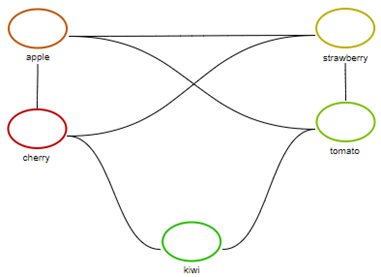
\includegraphics [scale=1] {my_folder/images/my/13}
	\caption{Пример результата, выдаваемого библиотекой Dracula Graph Library}
	\label{fig:13}
\end{figure}
\newpage
\begin{itemize}
\item Vis.js – размещает узлы не так, как хотелось бы (по принципу “упругого” физического движка), а так же сам вид визуализации не подходит для требуемого сервиса.
\end{itemize}
\begin{figure}[h]
	\center
	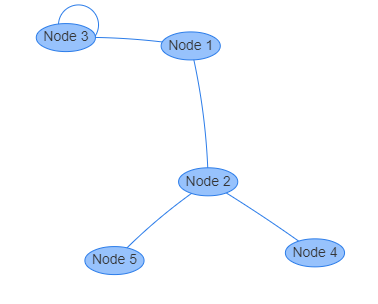
\includegraphics [scale=0.9] {my_folder/images/my/14}
	\caption{Пример результата, выдаваемого библиотекой Vis.js}
	\label{fig:14}
\end{figure}
\begin{itemize}
\item Cytoscape.js – так же размещает узлы хаотично.
\end{itemize}
\begin{figure}[h]
	\center
	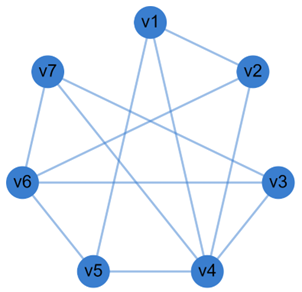
\includegraphics [scale=0.9] {my_folder/images/my/15}
	\caption{Пример результата, выдаваемого библиотекой Cytoscape.js}
	\label{fig:15}
\end{figure}
\begin{itemize}
\item JavaScript InfoVis Toolkit (JIT) - неплохо рисует деревья, но плохо рисует графы. Как и предыдущие библиотеки хаотично размещает узлы и ребра и не подходит по виду визуализации.
\end{itemize}
\begin{figure}[h]
	\center
	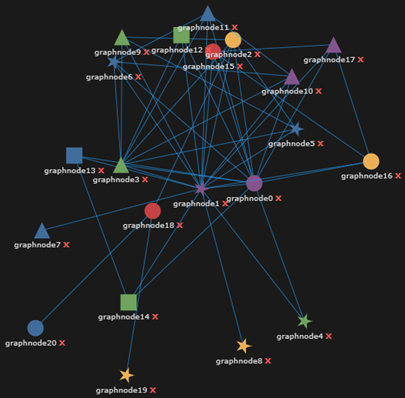
\includegraphics [scale=0.9] {my_folder/images/my/16}
	\caption{Пример результата, выдаваемого библиотекой JIT}
	\label{fig:16}
\end{figure}
\newpage
\begin{itemize}
\item D3.js – позволяет визуализировать очень много всего, но не то, что нужно для нашего сервиса. Тоже имеет “упругое” размещение и не обладает нужным видом.
\end{itemize}
\begin{figure}[h]
	\center
	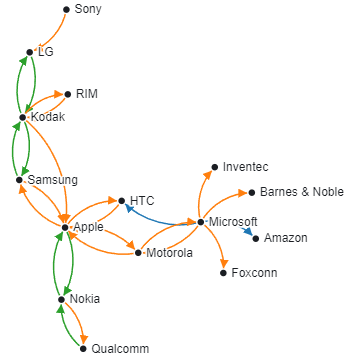
\includegraphics [scale=1] {my_folder/images/my/17}
	\caption{Пример результата, выдаваемого библиотекой D3.js}
	\label{fig:17}
\end{figure}
\begin{itemize}
\item Sigma.js - требует задания координат в XML и не обладает нужным видом.
\end{itemize}
\begin{figure}[h]
	\center
	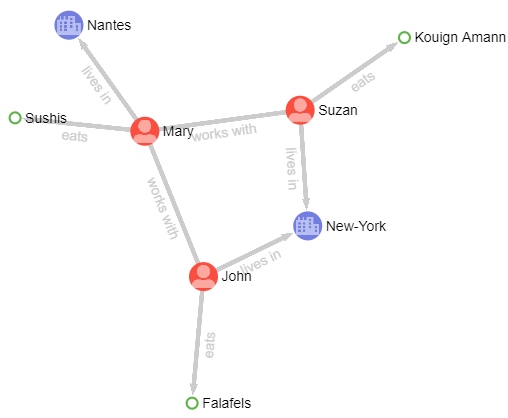
\includegraphics [scale=1] {my_folder/images/my/18}
	\caption{Пример результата, выдаваемого библиотекой Sigma.js}
	\label{fig:18}
\end{figure}
\begin{itemize}
\item Graphviz - был скомпилирован для Javascript с использованием Emscripten в формат WebAssembly. Существует в виде плагина к библиотеке D3.js. Умеет визуализировать графы с настраиваемым размещением и видом узлов, а также, отображает графы, описанные на языке DOT – универсальном языке описания графов.
Так же стоит рассмотреть вариант создания собственной визуализации.
\item Плюсы: достаточно компактное решение, которое делает именно то, что нужно
\item Минусы: сложная логика размещения и очень затратное по времени решение
\end{itemize}

Исходя из всего вышесказанного выбор пал на d3-graphviz, так как это наиболее подходящий вариант для нашего сервиса.
\section{Интерфейс взаимодействия с программой} \label{ch4:sec4}
Требуется создать интерфейс для взаимодействия с программой, для этого нужно определиться использовать или не использовать фреймворк.

Фреймворк – это инструмент для построения приложений. Обычно фреймворки определяют структуру приложения. Кроме того, они содержат множество уже готовых модулей, упрощающих разработку. В случае с JavaScript фреймворки помогают писать декларативный код, а не императивный. При использовании фреймворка обычно используются сборщики проекта. Как правило, настройка сборщика по умолчанию уже включает в себя компилятор babel, а также минификацию HTML, CSS и JavaScript кода. Минификация уменьшает размер и количество подключаемых файлов, что положительно сказывается на времени загрузки страниц. Babel позволяет писать код на новых версиях JavaScript, и он будет преобразован в JavaScript более старых версий, что увеличивает поддержку браузерами. Кроме этого, фреймворки добавляют плагины к babel, что позволяет использовать синтаксические конструкции, которых нет в чистом JavaScript. Кроме того, фреймворки позволяют запускать сервер для разработки, благодаря которому происходит отслеживание изменений в коде в режиме реального времени, и все изменения видны в браузере сразу без перезагрузки страницы.

Таким образом, можно сделать вывод, что фреймворки ускоряют и упрощают процесс разработки. Минус фреймворка заключается в том, что его код также включается в сборку, из-за чего JavaScript кода, который нужно загрузить в браузер, становится больше, что в некоторой степени замедляет первоначальную загрузку страницы. Было принято решение использовать фреймворк.
\section{Выбор фреймворка} \label{ch4:sec5}
1.	React
\begin{itemize}
\item Плюсы: большое сообщество, множество дополнительных библиотек, самый популярный на сегодняшний день, использует Virtual DOM (что улучшает производительность)
\item Минусы: громоздкий синтаксис, относительная сложность освоения, плохо структурированная документация, нестрогая структура приложения
\end{itemize}

2.	Angular
\begin{itemize}
\item Плюсы: огромный, мощный фреймворк, встроенная строгая типизация, множество встроенных возможностей, строгая структура приложения, хорошая документация
\item Минусы: сложно освоить, не использует Virtual DOM, большой размер, излишний для небольших проектов
\end{itemize}

3.	Vue.js
\begin{itemize}
\item Плюсы: очень простой и лёгкий в освоении, использует Virtual DOM (что улучшает производительность), хорошая документация, достаточно популярный
\item Минусы: не очень развитое сообщество, нестрогая структура приложения
\end{itemize}

4.	Svelte
\begin{itemize}
\item Плюсы: минимальный размер выходного приложения, простой в освоении, максимально производительный код на выходе
\item Минусы: очень молодой, непопулярный проект, маленькое сообщество
\end{itemize}

Проанализировав плюсы и минусы различных фреймворков, было принято решение, что для создания визуализатора самым подходящим будет Vue.js. Для обращений к серверу решено использовать библиотеку axios, как самое популярное решение для подобных задач, а в качестве готовых стилей для оформления интерфейса выбран CSS-фреймворк bulma.
\section{Выводы по главе} \label{ch4:sec6}
В данной главе описана архитектура и были выбраны средства решения. При создании сервиса будет использована клиент-серверная архитектура с использованием фреймворка Spark на стороне сервера и фреймворка Vue.js на стороне клиента. В качестве дополнительных инструментов будут использоваться JavaParser на стороне сервера для парсинга кода, Gson для сериализации в JSON. На стороне клиента будут использоваться axios для сетевых запросов, bulma для оформления интерфейса, d3 и d3-graphviz для отрисовки деревьев и графов.\\
\begin{figure}[h]
	\center
	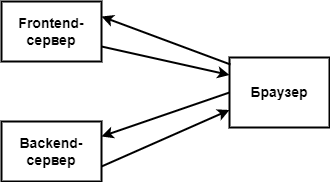
\includegraphics [scale=1] {my_folder/images/my/19}
	\caption{Схема работы сервиса} 
	\label{fig:19}  
\end{figure}

Когда пользователь открывает сервис в браузере, он обращается к Frontend серверу, откуда получает статические файлы HTML, CSS, JavaScript и другие, далее браузер строит по этим файлам страницу. Когда пользователь вводит код в интерфейсе, происходит запрос к Backend-серверу (его адрес прописывается в JavaScript от Frontend-сервера). Ответ от сервера обрабатывается браузером при помощи JavaScript-кода с Frontend-сервера.
\newpage














% не рекомендуется использовать отдельную section <<введение>> после лета 2020 года
%\section{Введение} \label{ch4:intro}

%Хорошим стилем является наличие введения к главе. Во введении может быть описана цель написания главы, а также приведена краткая структура главы. 
%	
%\section{Название параграфа} \label{ch4:sec1}
%
%\section{Название параграфа} \label{ch4:sec2}
%
%Пример ссылки на литературу \cite{avtonomova:fya,Peskov2004-ru,Kotelnikov2004-ru,Kotelnikov2004}.
%
%%\FloatBarrier % заставить рисунки и другие подвижные (float) элементы остановиться
%
%\section{Выводы} \label{ch4:conclusion}
%
%Текст выводов по главе \thechapter.
%
%%% Вспомогательные команды - Additional commands
%%
%%\newpage % принудительное начало с новой страницы, использовать только в конце раздела
%%\clearpage % осуществляется пакетом <<placeins>> в пределах секций
%%\newpage\leavevmode\thispagestyle{empty}\newpage % 100 % начало новой страницы